\documentclass{article}
\usepackage{amsmath}
\usepackage{graphicx}
\usepackage{graphics}
\usepackage{amssymb}
\usepackage{booktabs}
\usepackage{listings}
\usepackage{color}
\usepackage{caption}
\usepackage{subcaption}
\usepackage[margin=0.8in]{geometry}

\definecolor{dkgreen}{rgb}{0,0.6,0}
\definecolor{gray}{rgb}{0.5,0.5,0.5}
\definecolor{mauve}{rgb}{0.58,0,0.82}

\begin{document}
\title{Homework 2\\CS 5220}
\author{Lara Backer, Xiang Long, Saul Toscano}

\maketitle

%%%%%%%%%%%%%%%%%%%%%%%%%%%%%%%%%%%%%%%%%%%%%%%%%%%%%%%%%%%%%%%%%%%%%%%
\section*{Initial Profiling - Vtune}
\bigskip An initial profiling of the shallow wave code on the Totient cluster was done using Vtune, to identify which regions of the code took the longest time to run. This was done in order to target parallelization of the functions that took the longest time to complete. \\ \\
Figure \ref{fig1} displays the Vtune assessment of the overall program. The top three most time consuming functions are limited\_derivs, compute\_step, and compute\_fg\_speeds. 

 \begin{figure}[here]
  \centering
  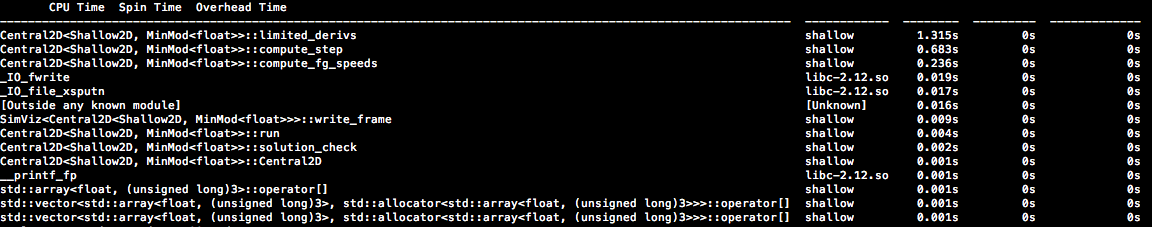
\includegraphics[width=0.8\linewidth]{vtune_orig_water_code.png}
  \caption{Most time consuming functions for shallow wave code on Totient cluster}
  \label{fig1}
\end{figure}

\noindent The function limited\_derivs is used to limit the estimation of the derivative of the fluxes by calling the limdiff function. Compute\_fg\_speeds is used to evaluate the fluxes at the cell centers. The compute\_step function is the seciton of the code that evaluates both the predictor and corrector calculations for the timestep. To see the time spent in each step using Vtune, the specific functions must be referenced. While this is not overly useful for the limited\_derivs function, which only performs the two limdiff calls, the in-depth timings for the other two most expensive functions are shown in Figures \ref{fig2} and \ref{fig3}.
 
 \begin{figure}[here]
  \centering
  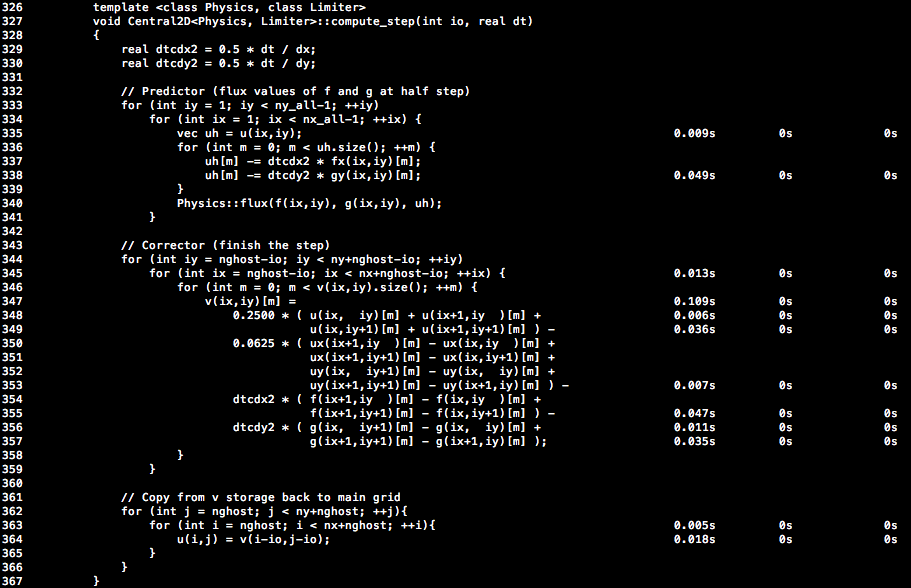
\includegraphics[width=0.8\linewidth]{vtune_origcode_computestep.png}
  \caption{compute step function timings}
  \label{fig2}
\end{figure}

\begin{figure}[here]
  \centering
  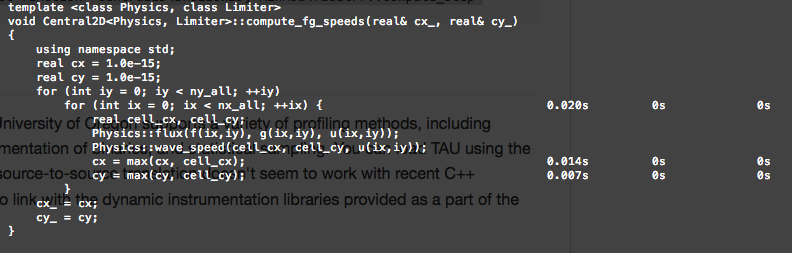
\includegraphics[width=0.8\linewidth]{compute_fgspeeds_orig_vtune.png}
  \caption{fgspeeds function timings}
  \label{fig3}
\end{figure}

There could be some performance gains in tuning the most expensive functions, however we chose to put most of our efforts into vectorization and parallelization as it is expected the gains here would be much more significant.

\section*{Vectorization}

One method of speeding up the code is to apply vectorization, applying operations to arrays instead of array sub elements, reducing the number of required computations. To apply vectorization to our code for instance, we grouped the fluxes into single arrays, specifying pointers to the locations of each flux, and indicating the strides required for each component.   

We drew ideas from the vectorization code produced by Prof. Bindel. In our code, the ipo\_out.optreport file output after compilation shows the sections that have be vectorized to improve efficiency. Our vectorization still uses the C++ standard library vector and iterator structures, which seem to have significant performance overheads. We are currently working on a version that uses pointers to reduce overheads in manipulating the data structure.

\section*{OpenMP Parallelization}
OpenMP can be used to further improve performance by multithreading, where each thread executes a section of the code independently. In C++, OpenMP uses \#pragmas to signify the parallelization of code. The pragma omp parallel, for instance, is used to fork threads to carry out the enclosed work. Additional pragmas can be used to specify sections of work, or splitting up loop iterations. 

The vectorization report was useful in identifying which loops should be targeted for parallelization. Loops that have data dependencies between iterations cannot be unrolled to work in parallel, so it would be futile to assign iterations to different threads. It was found that only the time-stepping loop in central2d was suitable for parallelization.

In order to test the relative performance of the original, vectorized and OpenMP-parallelized implementations, we performed a strong scaling study where the size $n$ of the side of the field is increased and the simulation times of each implementation is recorded. It was found that our vectorized code ran slower than the original implementation, and that with OpenMP it performed slower still. This could be due to overheads in our implementation, which we are aiming to fix for the final report. In particular the slowdown in OpenMP could be due to spawning too many threads to work on short computational tasks, where overheads in thread management will dominate.

\begin{figure}[here]
  \centering
  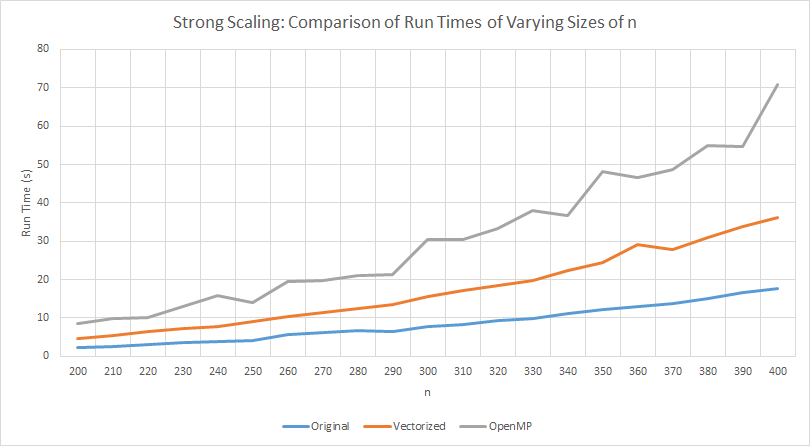
\includegraphics[width=0.8\linewidth]{strong-scaling.png}
  \caption{Strong scaling study}
  \label{fig4}
\end{figure}

We also performed a weak scaling study where we forced OpenMP to use between 1 to 12 threads, and the run times of these configurations were tested against the original \"unlimited\" setting where it was up to OpenMP how many threads to spawn. We found that with fewer threads performance was actually better, perhaps due to eliminating overheads in managing many threads. However there is clearly much more room for improvement in both the vectorization and parallelization performance.

\begin{figure}[here]
  \centering
  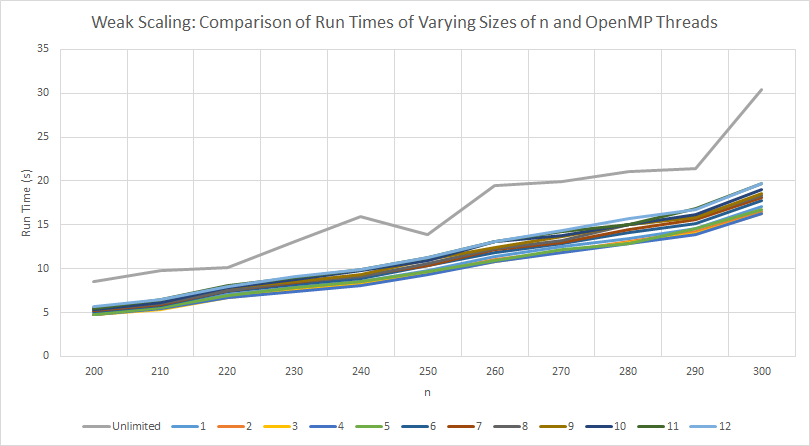
\includegraphics[width=0.8\linewidth]{weak-scaling.png}
  \caption{Weak scaling study}
  \label{fig4}
\end{figure}

\section*{Domain Decomposition}
The method best suited to parallelize the shallow water problem is domain decomposition. For this method, the overall domain is split and solved for on separate processors. Communications between processors are needed to solve for `ghost cells' that overlap neighboring domains. However, communications can overtake the domain computations in cost, depending on the number of processors and communications compared to the domain size that each processor has to solve, so scaling trials must be employed to determine the optimal problem size per processor. We are working on investigating this area for our final report.
\end{document}